\documentclass[11pt,a4paper,twocolumn]{article}
\usepackage[margin=2.2cm]{geometry}
\usepackage{times}
\usepackage{latexsym}
\usepackage[utf8]{inputenc}
\usepackage{booktabs}
\usepackage{enumitem}
\usepackage[hidelinks]{hyperref}
\usepackage{titlesec}
\usepackage[numbers]{natbib}
\usepackage{graphicx}
\usepackage{multirow}

\titleformat{\section}{\normalfont\large\bfseries\uppercase}{\thesection}{1em}{}
\titleformat{\subsection}{\normalfont\large\bfseries}{\thesubsection}{1em}{}

\title{\textbf{Q-Squeeze: A Comparative Study of Unstructured Pruning and Structured Pruning on Qwen 3.5}}

\author{
  \textbf{Jakub Sudoł} \\ \texttt{sudol.jak@gmail.com} \and
  \textbf{Hubert Szymański} \\ \texttt{hubertszym4@gmail.com} \and
  \textbf{Franciszek Wrzosek} \\ \texttt{fw.wrzosek@gmail.com} \\
  \\
  \textit{Supervisor: Jakub Krajewski}
}

\date{}

\begin{document}
\maketitle

\begin{abstract}
As Large Language Models (LLMs) grow in complexity, the demand for efficient deployment on hardware with limited resources increases. This report presents a comprehensive study on compressing the Qwen 3.5-4B model. We compare three distinct one-shot pruning paradigms: unstructured weight pruning via the Wanda algorithm, structured layer dropping via ShortGPT, and structured width pruning of attention heads and MLP dimensions. Our primary objective is to evaluate how these compression methods impact the model's performance relative to the original architecture, specifically focusing on the preservation of mathematical reasoning (GSM8K) and general multitask language understanding (MMLU). We demonstrate that while unstructured pruning effectively maintains reasoning capabilities even at 30\% sparsity, structured approaches suffer catastrophic performance degradation at similar compression rates in a zero-shot setting.
\end{abstract}

\section{Introduction}
The deployment of Large Language Models (LLMs) is heavily constrained by VRAM availability and inference latency. While efficient architectures like \textbf{Qwen 3.5-4B} can typically run on mid-range GPUs, reducing their memory footprint remains highly beneficial. Lowering VRAM usage allows for larger batch sizes, longer context windows, and improved accessibility on consumer-grade hardware, where memory overhead can otherwise become a bottleneck.

This report evaluates and compares fundamentally different approaches to identifying and exploiting redundancy in state-of-the-art small LLMs. Unstructured pruning methods like Wanda target individual weights throughout the network based on magnitude and activation context, preserving the physical shape of tensors but zeroing out elements. In contrast, structured pruning methods such as ShortGPT and width pruning physically alter the model architecture by removing entire redundant layers or slicing attention heads and MLP intermediate dimensions. 

Our goal is to evaluate which method maintains a better "Efficiency Frontier" between model size and performance. We focus our evaluation on \textbf{Mathematical Reasoning (GSM8K)} and \textbf{Multitask Language Understanding (MMLU)} to observe how significantly compression affects logical coherence and knowledge retention compared to the original, uncompressed model.

\section{Related Work}
Our study builds on recent advancements in post-training compression of language models. A primary motivation for exploring one-shot pruning comes from research by \citet{muralidharan2024compact}, which demonstrated that pruning and distillation pipelines can effectively downsize LLMs while maintaining high quality. 

For weight-level compression, we employ \textbf{Wanda} (Weight and Activation) \cite{sun2023wanda}, an algorithm that prunes weights based on the product of their magnitude and the norms of their corresponding input activations. This process utilizes a small "calibration set" to observe which neurons are most active during inference. 

For structured compression, we investigate two methods. The first is \textbf{ShortGPT} \cite{men2024shortgpt}, which identifies and drops redundant layers based on "Block Influence" metrics,
effectively reducing the model's depth. The second is \textbf{Width Pruning}, an activation-based approach that ranks and physically removes attention heads and MLP neurons. This aligns with recent findings that suggest width pruning can be highly effective when coupled with distillation, though our study focuses on the zero-shot degradation before any retraining.

\section{Pruning Methodologies}
The primary model investigated is \textbf{Qwen 3.5-4B}, a state-of-the-art dense model that strikes a balance between capabilities and parameter count. We aim to compress this model using three techniques:

\textbf{1. Wanda (Unstructured Pruning)}: Wanda evaluates each weight $W_{ij}$ in a linear layer based on the heuristic $S_{ij} = |W_{ij}| \times \|X_j\|_2$, where $X_j$ is the input activation norm. Weights with the lowest scores are set to zero. This method does not reduce the VRAM footprint during standard inference without specialized sparse kernels, but it acts as a strong baseline for theoretical capacity preservation.

\textbf{2. ShortGPT (Structured Layer Dropping)}: ShortGPT evaluates the redundancy of layers by calculating the cosine similarity between the input and output of a given layer block.
Layers that perform minimal transformations on the hidden states are deemed redundant and are entirely removed, reducing the depth of the model.

\textbf{3. Width Pruning (Structured Width Slicing)}: This method physically slices the weight matrices of Multi-Head Attention (MHA) query/key/value heads and MLP intermediate dimensions. By utilizing forward hooks to record L2 activation norms over a calibration dataset, we rank the most important heads and neurons. We align the pruning of attention heads to respect Grouped-Query Attention (GQA) divisibility constraints. The result is a physically smaller model that directly accelerates inference and reduces VRAM usage.

\section{Experimental Set-up}
Our experiments were conducted on the \textbf{Entropy Cluster}, utilizing \textbf{NVIDIA Titan V} and \textbf{RTX 2080 Ti} GPUs. 

\textbf{Calibration Setup}: For Wanda and ShortGPT, we utilized 128 calibration sequences, whereas for Width Pruning, we utilized 512 calibration sequences. The calibration dataset consisted of a 50/50 split sampled from the English C4 training set (\texttt{allenai/c4}) and the GSM8K training dataset. We configured the sequence length to 2048 tokens to compute the necessary activation norms and block influences in a single forward pass without excessive memory overhead.

\textbf{Evaluation Metrics}: We evaluated the pruned models using the \textbf{Language Model Evaluation Harness} (\texttt{lm-eval}). We specifically chose two demanding benchmarks:
\begin{itemize}[noitemsep]
    \item \textbf{MMLU} (Massive Multitask Language Understanding): To measure general knowledge retention across diverse subjects.
    \item \textbf{GSM8K} (Grade School Math 8K): To test the preservation of complex multi-step reasoning capabilities.
\end{itemize}

\textbf{Baselines}: We compare the pruned variants of Qwen 3.5-4B against two dense baselines: the uncompressed \textbf{Qwen 3.5-4B} itself, and the smaller native \textbf{Qwen 3.5-2B} model. The 2B model serves as a critical benchmark to determine if a pruned 4B model is more efficient than simply using a smaller, fully trained model. 

We pruned the Qwen 3.5-4B model at varying sparsity levels (10\%, 20\%, 30\%) for all three methods. We additionally evaluated Wanda up to 50\% sparsity to map out the degradation curve further; this extended evaluation was performed exclusively for Wanda as it presented the best and most promising results on the benchmarks.

\section{Results and Discussion}

The evaluation results on MMLU and GSM8K are summarized in Table~\ref{tab:results}. 

\begin{table*}[t]
\centering
\caption{Performance comparison of Qwen 3.5-4B under different pruning methods and sparsity levels. Baseline models are the dense Qwen 3.5-4B and Qwen 3.5-2B. Values represent accuracy.}
\label{tab:results}
\begin{tabular}{lcccccc}
\toprule
\textbf{Model / Pruning} & \textbf{Sparsity} & \textbf{MMLU Acc.} & \textbf{MMLU Std.} & \textbf{GSM8K Acc.} & \textbf{GSM8K Std.} \\
\midrule
Qwen 3.5-4B (Dense) & 0\% & 0.7439 & 0.0035 & 0.7521 & 0.0119 \\
Qwen 3.5-2B (Dense) & 0\% & 0.5924 & 0.0039 & 0.5754 & 0.0136 \\
\midrule
Wanda & 10\% & 0.7421 & 0.0035 & \textbf{0.7703} & 0.0116 \\
Wanda & 20\% & 0.7399 & 0.0035 & 0.6998 & 0.0126 \\
Wanda & 30\% & 0.7310 & 0.0035 & 0.6497 & 0.0131 \\
Wanda & 50\% & 0.6163 & 0.0039 & 0.6012 & 0.0135 \\
\midrule
ShortGPT (Layer Drop) & 9.37\% & 0.7353 & 0.0035 & 0.4185 & 0.0136 \\
ShortGPT (Layer Drop) & 18.75\% & 0.6646 & 0.0037 & 0.0447 & 0.0057 \\
ShortGPT (Layer Drop) & 28.25\% & 0.5532 & 0.0041 & 0.0273 & 0.0045 \\
\midrule
Width Pruning & 10\% & 0.5693 & 0.0040 & 0.3829 & 0.0134 \\
Width Pruning & 20\% & 0.4494 & 0.0041 & 0.2532 & 0.0120 \\
Width Pruning & 30\% & 0.3197 & 0.0039 & 0.0341 & 0.0050 \\
\bottomrule
\end{tabular}
\end{table*}

\subsection{Unstructured Pruning (Wanda)}
Wanda demonstrates remarkable robustness across all sparsity levels. At 10\% sparsity, the model's GSM8K accuracy surprisingly increases to 77.03\%, slightly outperforming the dense baseline (75.21\%). This suggests that minor unstructured weight removal may provide a slight regularization effect or remove noisy activations that hinder mathematical reasoning. Even at a high sparsity of 30\%, Wanda maintains an MMLU score of 0.7310 and a GSM8K score of 0.6497, significantly outperforming the dense Qwen 3.5-2B model. This indicates that unstructured sparsity effectively preserves the distributed knowledge representations and reasoning pathways within the network.

\subsection{Structured Layer Dropping (ShortGPT)}
While ShortGPT performs reasonably well on MMLU at low sparsity (10\% removal yields 0.7353 accuracy), it struggles severely on complex reasoning tasks.
At roughly 10\% layer drop, GSM8K accuracy collapses from 0.7521 to 0.4185. At roughly 20\% and 30\% depth reduction, the model completely loses its ability to perform grade-school math,
with accuracy plummeting to 0.0447 and 0.0273, respectively.
This catastrophic degradation is consistent with the findings reported in \cite{men2024shortgpt}, where the authors observed a similar effect for 7B models after removing 25\% of their layers and left its underlying causes as an open question.
In our case, the degradation on GSM8K suggests that logical reasoning may be highly sequential and dependent on specific layer transformations.
Removing entire blocks may therefore disrupt the reasoning process required for GSM8K, even if general knowledge, as measured by MMLU, decays more gracefully. The block influence metric computed across all layers, which dictates the layers selected for removal, is visualized in Figure~\ref{fig:bi_plot}.

\subsection{Structured Width Pruning}
Width pruning proved to be the most destructive zero-shot compression method in our experiments. Even at a minimal 10\% sparsity, MMLU drops to 0.5693, and GSM8K falls to 0.3829.
By 30\% sparsity, the model's capabilities are almost entirely eliminated. The physical slicing of attention heads and MLP dimensions suddenly breaks the
specialized routing and representation capacities of the model. 

Comparing these results to the literature on compact language models \cite{muralidharan2024compact}, it is evident that structured width pruning should not be used as a standalone
zero-shot technique. While unstructured pruning like Wanda can be applied directly, structured pruning methods require subsequent lightweight
retraining or knowledge distillation to repair the severed representation pathways and restore performance.

\section{Conclusions}
In this report, we investigated the impact of unstructured and structured pruning on the Qwen 3.5-4B model. Our findings highlight a stark contrast between theoretical capacity reduction and structural disruption. Wanda's unstructured approach preserves both general knowledge and logical reasoning remarkably well, proving to be a safe zero-shot compression technique. Conversely, structured methods like ShortGPT and Width Pruning result in severe zero-shot degradation, particularly on reasoning tasks, emphasizing that physical architectural modifications require subsequent retraining or distillation to be viable.

\begin{thebibliography}{9}
\bibitem[Muralidharan et al.(2024)]{muralidharan2024compact} Muralidharan, S., et al. (2024). Compact Language Models via Pruning and Knowledge Distillation. \textit{arXiv:2408.11796}.
\bibitem[Sun et al.(2023)]{sun2023wanda} Sun, M., et al. (2023). A Simple and Effective Pruning Approach for Large Language Models. \textit{arXiv:2306.11695}.
\bibitem[Men et al.(2024)]{men2024shortgpt} Men, X., et al. (2024). ShortGPT: Layers in Large Language Models are More Redundant Than You Expect. \textit{arXiv:2403.03853}.
\end{thebibliography}

\onecolumn
\appendix
\section{Appendix}

\begin{figure}[h]
    \centering
    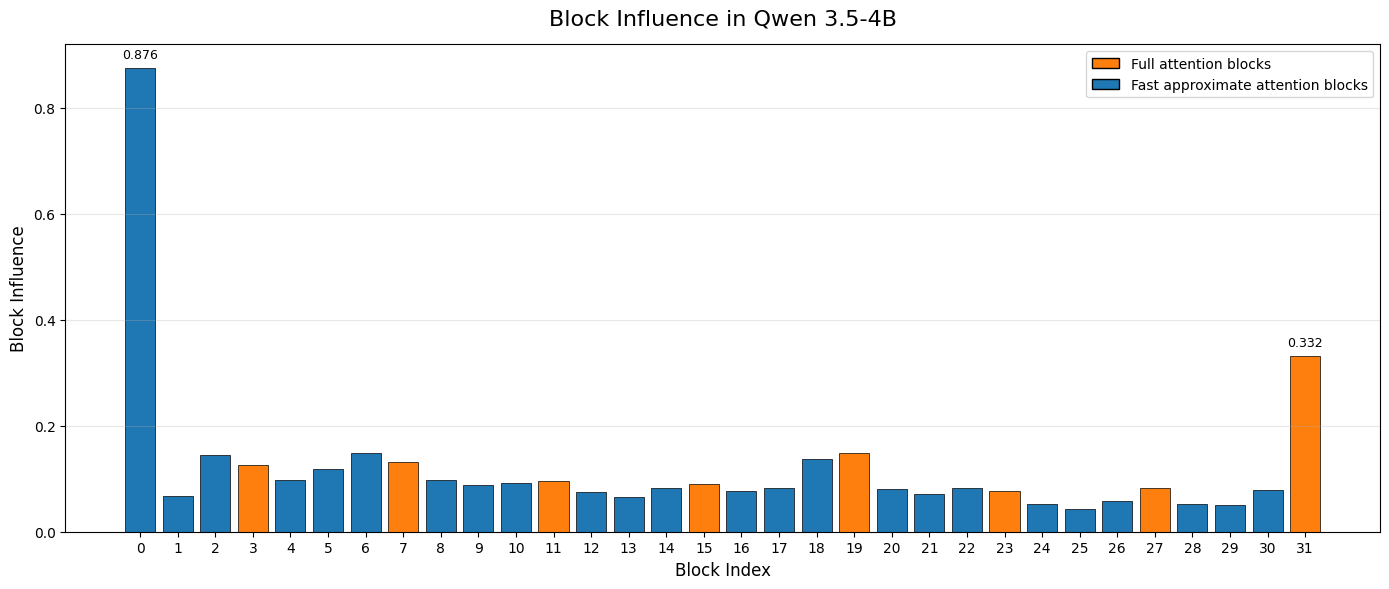
\includegraphics[width=0.8\linewidth]{../plots/BI_plot.png}
    \caption{Block Influence across layers in the Qwen 3.5-4B model. Layers with the lowest influence are targeted for removal in the ShortGPT method.}
    \label{fig:bi_plot}
\end{figure}

\end{document}
